\UseRawInputEncoding
\documentclass{elteikthesis}

\title{Methcodus}
\date{2020}
\author{Fityó Csaba}
\degree{programtervező informatikus BSc}
\supervisor{Nagy Sára}
\affiliation{mesteroktató}
\extsupervisor{Czeller Ildikó}
\extaffiliation{adattudós}
\university{Eötvös Loránd Tudományegyetem}
\faculty{Informatikai Kar}
\department{Algoritmusok és Alkalmazásaik}
\departmentSecondLine{Tanszék}
\city{Budapest}
\logo{elte-crest}

\begin{document}

	\documentlang{magyar}

	\maketitle

	\tableofcontents

	\chapter{Bevezetés}

		\section{Motiváció}
			Manapság számtalan lehetőség van, ha valaki programozni szeretne tanulni, ebből rengeteg lehetőség könnyen hozzáférhető a legtöbb ember számára. Ha csak az internet adta lehetőségeket vesszük figyelembe, léteznek oktató leírások, oktatóvideók, kérdések és válaszok, és még sok más lehetőség.

			Ezeket a lehetőségeket még tovább lehet bővíteni. Hasznos lehetne egy olyan platform, amely programozási készségek fejlesztésére alkalmas, egyszerűen használható, de sokoldalú. Segítségével a felhasználónak lehetősége lenne egyszerre kisebb programozási feladatokat megoldani, szoftverfejlesztési módszereket tanulni vagy gyakorolni, illetve programozási nyelveket gyakorolni vagy egy újban kipróbálni magát, miközben visszajelzést kap, hogy ezeket megfelelően használja-e. Ha ezeket egyszerre szeretné elérni valaki, akkor jellemzően több forrásból kell táplálkoznia és még úgy sem lehet biztos magában; megtanul valahol egy szoftverfejlesztési módszert és keres máshol egy feladatot amelyet meg szeretne oldani ezzel a módszerrel. Sajnos nem feltétlenül talál a feladathoz megoldást az általa választott nyelven, és abban sem lehet biztos, hogy a módszert jól alkalmazta.
			
			Egy olyan szoftver, amely mindezt tudja, kezdő és tapasztalt programozóknak is hasznos lehet. A kezdőbbek az algoritmizálási képességeiket, logikájukat fejleszthetik, új szoftverfejlesztési módszereket sajátíthatnak el és programozási nyelveket próbálhatnak ki. A tapasztaltabbak frissen tarthatják ezen készségeiket, újakat tanulhatnak, vagy szórakozásként is használhatják. A cél egy ilyen szoftver létrehozása.

		\section{Feladatleírás}
		TODO (röviden, közérthetően)

	\chapter{Felhasználói dokumentáció}
		
		\section{Használati követelmények}
		TODO (rendszerkövetelmények, tudásbeli követelmények, angol nyelv, elérési link)
		
		\section{Alkalmazás funkciói}
		TODO (minden funkció leírása képernyőképekkel, külön regisztrált és nem regisztrált felhasználóra, külön helyes és hibás használatra)
		
		\section{Szoftverfejlesztési módszerek}
		Az alkalmazás által feladatmegoldáskor támogatott szoftverfejlesztési módszerek a következők:
		\subsubsection{Tesztvezérelt fejlesztés}
			A tesztvezérelt fejlesztés (TDD) \cite{tdd} egy szoftverfejlesztési technika, amely a szoftver fejlesztésének folyamatát tesztek írásával irányítja. A módszert Kent Beck fejlesztette ki a 90-es évek végén. Alkalmazásához három egyszerű lépést kell sorban, ismételten elvégezni; teszt írása, kód írása és refaktorálás. Teszt írásakor egyetlen új tesztet kell írni. Ennek a tesztnek el kell buknia az akkori implementáción, vagyis olyan tesztet kell írni, amely egy, még nem lefejlesztett funkcionalitás meglétét teszteli. Kód írásakor olyan módon kell kiegészíteni az implementációt, hogy az újonnan írt teszt, illetve a korábbi tesztek is átmenjenek. Refaktoráláskor hozzá szabad nyúlni a tesztekhez is és az implementációhoz is. Ezt olyan módon kell tenni, hogy nem változtatunk az implementáció, illetve a tesztek működésén. A kód olvashatóságának és jól strukturáltságának fenntartására szolgál ez a lépés.
			
			Ennek a módszernek előnye, hogy a kódunk jelenlegi működése garantálva lesz és továbbfejlesztéskor hamar kiderül, ha egy adott változtatás elront egy meglévő funkcionalitást. További előny, hogy teszt írásakor eszünkbe juthat olyan eset is, amely nem jutna eszünkbe akkor, ha először az implementációt írnánk meg, így lehetséges, hogy egy több esetet lefedő, jobban működő programot kapunk eredményül.

		\subsubsection{Páros programozás}
			A páros programozás \cite{pairprogramming} egy olyan tevékenység, amely során két ember dolgozik ugyanannak a programozási feladatnak a megoldásán, jellemzően ugyanazon a számítógépen. Ez egy nagyon kollaboratív módja a programozásnak, sok kommunikációt igényel. A pár tagjai nem csak magát a programozást csinálhatják együtt, hanem sok esetben együtt tervezik meg a munkát is, illetve munka közben megbeszélik ötleteiket a jobb megoldás érdekében. Sokféle páros programozási stílus létezik. A legegyszerűbb, strukturálatlan stílusban nincsenek szabályok, a pár tagjai a munka során megbeszélik, hogy éppen kinél legyen a billentyűzet. Az összetettebb stílusok közé tartozik például a "driver-navigator" és a "ping pong".

		\subsubsection{Ping pong}
			A ping pong \cite{pairprogramming} egy páros programozási stílus. Egyesíti a tesztvezérelt fejlesztés és a páros programozás elemeit. Első lépésben a pár egyik tagja ír egy új, elbukó tesztet. Második lépésként a pár másik tagja kiegészíti az implementációt úgy, hogy kielégítse az új tesztet is, azután refaktorálhatja a kódokat ha szeretné, végül pedig ír egy új, elbukó tesztet. Ezután a pár első tagja ismét megcsinál egy kód-refaktor-teszt lépéssorozatot, és így tovább.

	\chapter{Fejlesztői dokumentáció}

		\section{Probléma specifikáció}
		TODO (célok meghatározása fejlesztői szemmel)

		\section{Tervezés}

			\subsection{Használati esetek}
			TODO (használati eset diagram)
			
			\subsection{Felület terv}
			TODO (mockupok a felületről?)
			
			\subsection{Architektúra terv}
				A specifikációban szereplő igényeinket kiválóan kielégíti egy webes alkalmazás, amelynek architektúrája 3 komponensből áll. Az architektúra tartalmaz egy adatbázist, egy kiszolgálót, amely a szerver alkalmazást működteti, illetve egy másik kiszolgálót, amely a kliens alkalmazásért felel. A szerver alkalmazás egy REST elvekre épített webes API, ami az adatbázis felhasználásával megvalósítja az alkalmazás szerveroldali felületét. A kliens alkalmazás egy SPA, ami HTTP kéréseken keresztül fog kommunikálni a szerver alkalmazással. A kliens alkalmazást alkotó statikus fájlok elérését egy külön kiszolgáló biztosítja. Ezek a komponensek egy-egy Docker konténerben vannak izolálva egymástól és a külvilágtól.
				
				\begin{figure}[H]
					\centering
					\includegraphics[scale=0.3333]{architecture-diagram}
					\caption{Az alkalmazás architektúra terve}
				\end{figure}
			TODO (rövid leírás a technikai megvalósításról)
		
		\section{Szerver architektúra}

			\subsection{Authentikáció}
			TODO (annak folyamata)
			
			\subsection{Adatbázis}
			TODO (modellek leírása és ábra, kapcsolatok)
			
			\subsection{Végpontok}
			TODO (leírásuk, működésük, kérés és válasz tartalma, hibalehetőségek)
			
			\subsection{WebSocket üzenetek}
			TODO (leírásuk, működésük, oda- vissza üzenetek tartalma, hibalehetőségek)
			
			\subsection{Felhasznált technológiák}				
				\subsubsection{Node.js}
					A Node.js \cite{nodejs} egy nyílt forráskódú, platformfüggetlen JavaScript futtatókörnyezet. Node.js a V8 JavaScript motort használja, ami a Google Chrome magja, ezért nagyon jó teljesítménnyel tud működni. Minden Node.js alkalmazás egy folyamatként, egy szálon fut. Nem hoz létre új szálakat az új kérések miatt, ehelyett aszinkron I/O műveleteket kínál a szabványos könyvtárában, amik meggátolják, hogy a JavaScript kódok blokkolják a program futását. Amikor a Node.js egy I/O műveletet hajt végre, mint például olvasás a hálózatról, egy adatbázisból vagy a fájlrendszerből, a szál blokkolása és CPU ciklusok várakozással való pazarlása helyett akkor folytatja a műveletet, amikor visszakapja a választ. Node.js-ben az új ECMAScript szabványok minden probléma nélkül használhatóak, mert a szerveroldalon való futtatás miatt nem kell arra várni, hogy a felhasználók frissítsék a böngészőjüket, rajtunk múlik hogy a szabvány melyik verzióját szeretnénk használni.
				
				\subsubsection{TypeScript}
					A TypeScript \cite{typescript} egy nyílt forráskódú programozási nyelv, ami JavaScripten alapul, azt statikus típusdefiníciókkal egészíti ki. TypeScriptben a típusok opcionálisak, ebből következőleg minden érvényes JavaScript kód egyben érvényes TypeScript kód is. A nyelv által adott típusmegkötések a fejlesztés során nyújtanak segítséget, illetve dokumentálják a kódot, de közvetlenül nem futtathatók ezek a kódok. A TypeScriptben írt kódokat JavaScript kódokká alakítja át a TypeScript fordító, ezután lesznek futtathatók például böngészőben vagy Node.js-ben.
				
				\subsubsection{NestJS}
					A NestJS \cite{nestjs} egy nyílt forráskódú keretrendszer hatékony, skálázható, szerveroldali Node.js alkalmazások építésére. TypeScriptben és JavaScriptben való kódolásra is lehetőséget ad, kombinálja az objektumorientált programozás, a funkcionális programozás és a reaktív programozás elemeit. A motorháztető alatt a NestJS alapértelmezetten az Expresst használja HTTP szerver keretrendszerként.
				
				\subsubsection{REST}
					A REST (REpresentational State Transfer) \cite{rest} ajánlások, módszerek halmaza webes szolgáltatások programozására. Egy módszert ír le két számítógép (szerver és kliens) HTTP kapcsolaton keresztüli kommunikációjára. Előírja, hogy állapotmentes legyen a kommunikáció, vagyis a kliens által küldött kérésnek minden szükséges információt tartalmaznia kell ahhoz, hogy válaszolni lehessen rá. A REST-nek megfelelő kérések idempotensek, azaz ugyanazt a kérést többször egymás után elküldve ugyanazt a választ kell kapni, továbbá a válaszoknak tartalmaznia kell, hogy a kérés gyorsítótárazható-e vagy nem. A kommunikációnak olyan módon kell rétegezettnek lennie, hogy a kliensek szemszögéből ne derüljön ki, hogy egy közbenső géppel kommunikálnak vagy az aktuális szerverrel.
				
				\subsubsection{MongoDB}
					A MongoDB \cite{mongodb} egy nyílt forráskódú, általános célú, dokumentum alapú elosztott adatbázis szoftver. Elérhető hosztolható változatban, illetve felhőben futó változatban is. Hivatalosan több mint 10 programozási nyelvet támogat, egyszerűen megtanulható, de minden adottsága megvan komplex követelmények teljesítéséhez. Az adatokat rugalmas, JSON-szerű dokumentumokban tárolja, a dokumentumok modellje az alkalmazások kódjában lévő objektumokra illeszkedik, ezért könnyű vele dolgozni.

			TODO (mit tud, mire és hogyan használom: TSLint, Ubuntu, Java, JavaScript, JUnit, Jasmine, Babel, Core.js, WebSocket, Socket.io, Passport, JWT)
			
			\subsection{Kód felépítése}
			TODO (mappaszerkezet, rétegek)
		
		\section{Kliens architektúra}

			\subsection{Authentikáció}
			TODO (annak folyamata)
			
			\subsection{Képernyők}
			TODO (leírásuk, komponenseik)
			
			\subsection{Komponensek}
				\subsubsection{Code Editor}
				A Code Editor komponens valósítja meg az alkalmazásban használt kódszerkesztőt. A cél egy olyan kódszerkesztő létrehozása, amely nagyban megkönnyíti a különböző szoftverfejlesztési módszerek támogatását. Ezt használjuk fel a feladatok megoldásánál bármely módszer választása esetén, illetve a saját megoldások listázásánál is. A komponens a CodeMirror nevű kódszerkesztőre épül, néhány funkcióját átveszi, néhányat pedig testreszabja az alkalmazás igényeire. Lehetőséget nyújt az alkalmazás által támogatott programozási nyelvek használatára, a szerkesztő kezdeti tartalmának beállítására és jelenlegi tartalmának lekérésére. Kiegészítőket használ fel, amelyekkel például képes keresni, kikommentelni bizonyos sorokat és kiemelni a kijelöléssel egyező részeket a szövegben.
				
				Lehetőség van különböző szerkesztési módok beállítására, azok közötti váltásra:
				\begin{itemize}
					\item Normál mód: ez az alapértelmezett mód, ebben a módban tudja a felhasználó szerkeszteni a tartalmat.
					\item Csak olvasható mód: a tartalom szerkesztése le van tiltva, csak annak kijelölése és másolása van engedélyezve ebben a módban. A kurzor villogásának és egyéb vizuális kódszerkesztési tulajdonságoknak a kikapcsolása segíti a felhasználót a mód megkülönböztetésében.
					\item Inaktív mód: ebben a módban a kód szerkesztése és kijelölése is le van tiltva. A szerkesztő elhalványulása és tiltó jelzés megjelenítése jelzi a felhasználónak, hogy jelenleg nem használhatja a szerkesztőt.
				\end{itemize}

				A komponens lehetővé teszi a szerkesztőben történő változásokba való befolyást. Azt szeretnénk, hogy bármely változást teljesen meg tudjunk szakítani, illetve bármikor végre tudjunk hajtani változásokat egyszerűen programozható módon. Ezt a CodeMirror ehhez kapcsolódó eseményeire való feliratkozásokkal és azok megfelelő kezelésével tudjuk megtenni. Ezek segítségével minden változást megszakítunk, összegyűjtjük a megszakított változtatás későbbi végrehajtásához szükséges adatokat, és azokkal kiváltunk egy saját eseményt. Erre az eseményre feliratkozva egyszerűen, egységes módon meg tudjuk szakítani a szerkesztésre irányuló eseményeket, vagy tovább tudjuk engedni azokat végrehajtásra, vagy eltárolhatjuk a kapott adatokat a változás későbbi végrehajtásához. Amennyiben nem szakítjuk meg az eseményt, a változás végrehajtódik. A támogatott változások a következők:
				\begin{itemize}
					\item Kijelölés változás: a mutatóeszközökkel (például egérrel) és érintőképernyővel végzett kijelölés változások tartoznak ide. Ennek a változásnak a megszakítása nem támogatott az eredeti eseményben, ezért az általunk kiváltott eseményben láthatatlanul visszaállítjuk a kijelölést az előző állapotra. 
					\item Tartalom változás: ide tartoznak a billentyűleütésekből következő tartalom változások, illetve a kivágás és beillesztés. Abban az esetben, ha egyszerre több kijelölés van a tartalom változás idejében, akkor az eredeti eseményben minden kijelölésben történő változásról külön eseményt kapunk. A saját eseményben ezeket összevonjuk, csak egy eseményt váltunk ki. 
					\item Billentyűparancs: az olyan, billentyűzettel bevihető parancsok tartoznak ide, mint előre- és visszavonás, kódformázási és kurzor mozgatási parancsok. Billentyű leütésekor ellenőrizzük, hogy egy billentyűparancshoz kapcsolódó billentyűkombináció lett-e leütve, ekkor figyelembe vesszük a beépített, illetve az általunk hozzáadott kombinációkat is.
				\end{itemize}
				A CodeMirror az alváltozásokról is küld eseményeket, vagyis például a billentyűleütések utáni kijelölés változásokról, vagy a billentyűparancsok utáni tartalom változásokról. A komponensben ezeket összesítjük, a saját eseményben csak a kiváltó eseménnyel foglalkozunk a változások egységes, egyszerű kezelése érdekében.

			TODO (leírásuk, működésük, hibalehetőségek)
			
			\subsection{Felhasznált technológiák}
				\subsubsection{Angular}
					Az Angular \cite{angular} egy nyílt forráskódú, platformfüggetlen, kliensoldali JavaScript keretrendszer, amely TypeScriptben való fejlesztésre ad lehetőséget. Használatával webes, mobil és asztali alkalmazások is fejleszthetők, támogatja a SPA-k fejlesztését is. Egy Angular alkalmazás általában sok apró komponensből épül fel, egy komponens tartalmazza magát a forráskódot (TypeScript), a megjelenést (HTML) és a stílust is (CSS). Kétirányú adatkötést használ, aminek köszönhetően automatikusan követi a felhasználói felület az adattár változásait, illetve az adattár a felhasználói felület változásait.
			
				\subsubsection{SPA}
					A SPA (Single-Page Application) \cite{spa} egy webalkalmazás implementáció, amely egyetlen oldalbetöltéssel letölti az alkalmazás működéséhez szükséges összes JavaScript, HTML és CSS fájlt, és az alkalmazás különböző tartalmainak lekérésekor mindig csak az oldal tartalma módosul a teljes újratöltés helyett. Ez megengedi a felhasználóknak azt, hogy anélkül használjanak weboldalakat, hogy közben új oldalakat kellene letölteni a szerverről, ami teljesítménybeli javulást és dinamikusabb felhasználói élményt hozhat, viszont nagyobb erőfeszítést igényel egy ilyen alkalmazás fejlesztése és karbantartása.
			
				\subsubsection{CodeMirror}
					A CodeMirror \cite{codemirror} egy nyílt forráskódú, sokoldalú, JavaScriptben írt szövegszerkesztő, amely böngészőkben fut. Leginkább forráskódok szerkesztésére van specializálva, több mint 100 programozási nyelvet támogat. Rendelkezik megszokott kódszerkesztési tulajdonságokkal, mint például szintaxiskiemelés, előre- és visszavonás, billentyűparancsok. Ezek további, összetettebb tulajdonságokkal bővíthetők, ilyen például a keresés és az automatikus kódkiegészítés. Gazdag API-jának és CSS alapú stílusrendszerének köszönhetően szabadon testreszabható, illetve kiegészíthető új funkcionalitással.

				\subsubsection{Express}
					Az Express \cite{express} egy nyílt forráskódú, minimalista keretrendszer szerveroldali Node.js alkalmazások építésére, amely a Node.js beépített HTTP moduljára épül. Nagyon rugalmasan, sokféleképpen használható, nem írja elő, hogy hogyan kell felépíteni, strukturálni a vele írt alkalmazásokat.

			TODO (mit tud, mire és hogy használom: PrimeNG)
			
			\subsection{Kód felépítése}
			TODO (komponensdiagram, mappaszerkezet, rétegek)
		
		\section{Komponensek közti kommunikáció}
		TODO (szekvenciadiagram egy funkcióra, opcionális)

		\section{A tesztelő rendszer működése}
			Az alkalmazás leglényegesebb része a tesztelő rendszer. A felhasználók által megoldandó programozási feladatok megoldása közben, illetve azok beküldésekor nyújt támpontot számukra azáltal, hogy kiértékeli a megoldásukat és egységes formájú jelentést készít annak állapotáról. Akár tesztvezérelt fejlesztéssel oldja meg a felhasználó a feladatot, akár nem, ez a rendszer felel a megoldás teszteléséért. A tesztelő rendszer a szerveroldalon található, HTTP kapcsolaton keresztül folyik a kommunikáció. Megkapjuk a teszteléshez szükséges adatokat, elvégezzük a teszteket, utána pedig válaszolunk a teszteredményekkel.
			
			Miután megérkeznek HTTP kérésen keresztül a megfelelő adatok, elindítjuk a tesztelést külön folyamatban parancssori programként, a tesztelendő megoldás programozási nyelve szerinti, azon a nyelven írt tesztelő program indításával. Java esetén a \texttt{java}, JavaScript esetén pedig a \texttt{node} parancsot használjuk erre, a teszteléshez szükséges adatokat pedig környezeti változókon keresztül, szövegesen kapja meg a tesztelő. Miután a tesztelő elvégezte feladatát, tudatnia kell az eredményeket az őt hívó szülőfolyamattal. Sikeres tesztelés esetén kiírja a standard kimenetre a teszteredményeket. Hiba esetén kilépési kódokat használunk:
			\begin{itemize}
				\setlength\itemsep{-0.5em}
				\item[1:] a beküldött kódokban lévő szintaktikai hibát jelez
				\item[2:] a beküldött kódokban lévő fordítási hibát jelez
				\item[255:] egyéb, ismeretlen hiba
			\end{itemize}

			A tesztelő folyamat terminálásakor, a szülőfolyamatban kiolvassuk a standard kimenetet, illetve a kilépési kódot. Ezek alapján, illetve hiba esetén egy hibaüzenetet előállítva küldjük vissza a HTTP választ, ami alapján megjelenítjük a felhasználónak a megoldása állapotát. TODO (tesztelésnek a felületen lévő részeiről, egységes formátum alapú módszernél a validációról is írni)
		
			A tesztek futtatására két mód van. Az egyik módszer az egységteszt keretrendszer kódján alapuló tesztelés, másik pedig az egységes formátumon alapuló tesztelés. Mindkét módszer képes együttműködni Java és JavaScript nyelven írt kódokkal.

			\begin{figure}[H]
				\centering
				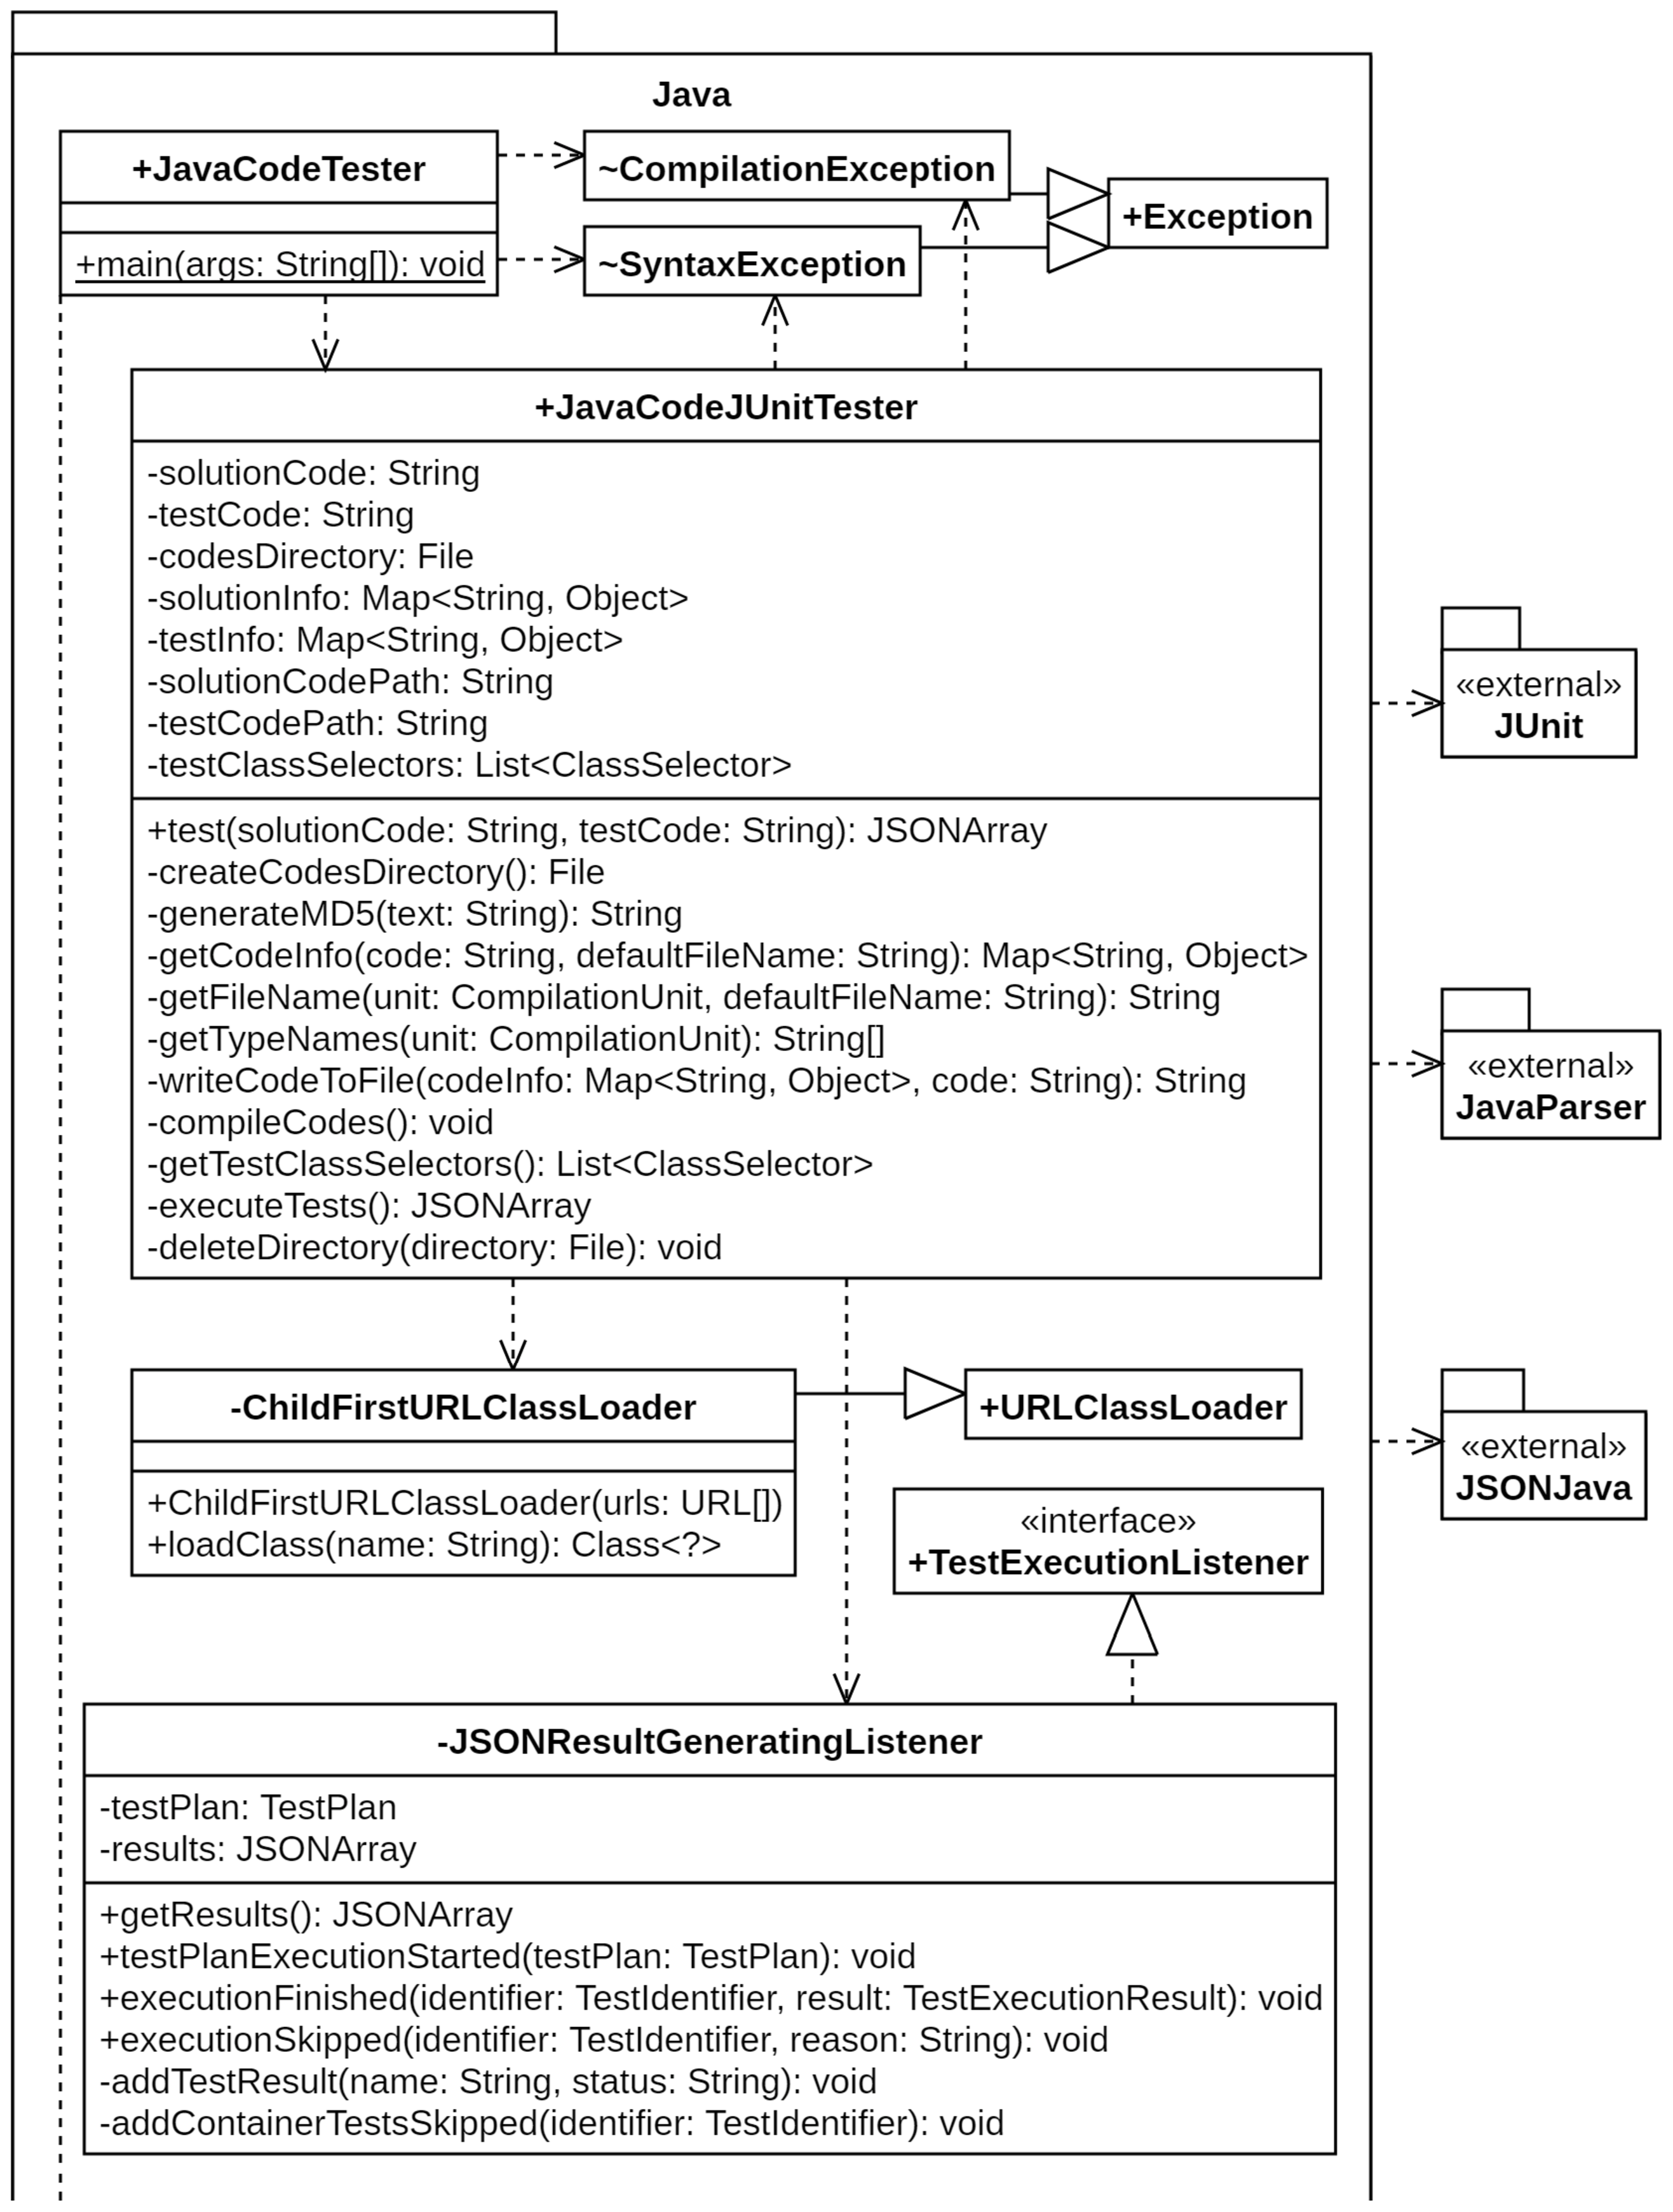
\includegraphics[scale=0.3333]{staruml/tester-system-class-diagram-1}
				\caption{A tesztelő rendszer osztálydiagramja - 1. rész}
			\end{figure}
			
			\begin{figure}[H]
				\centering
				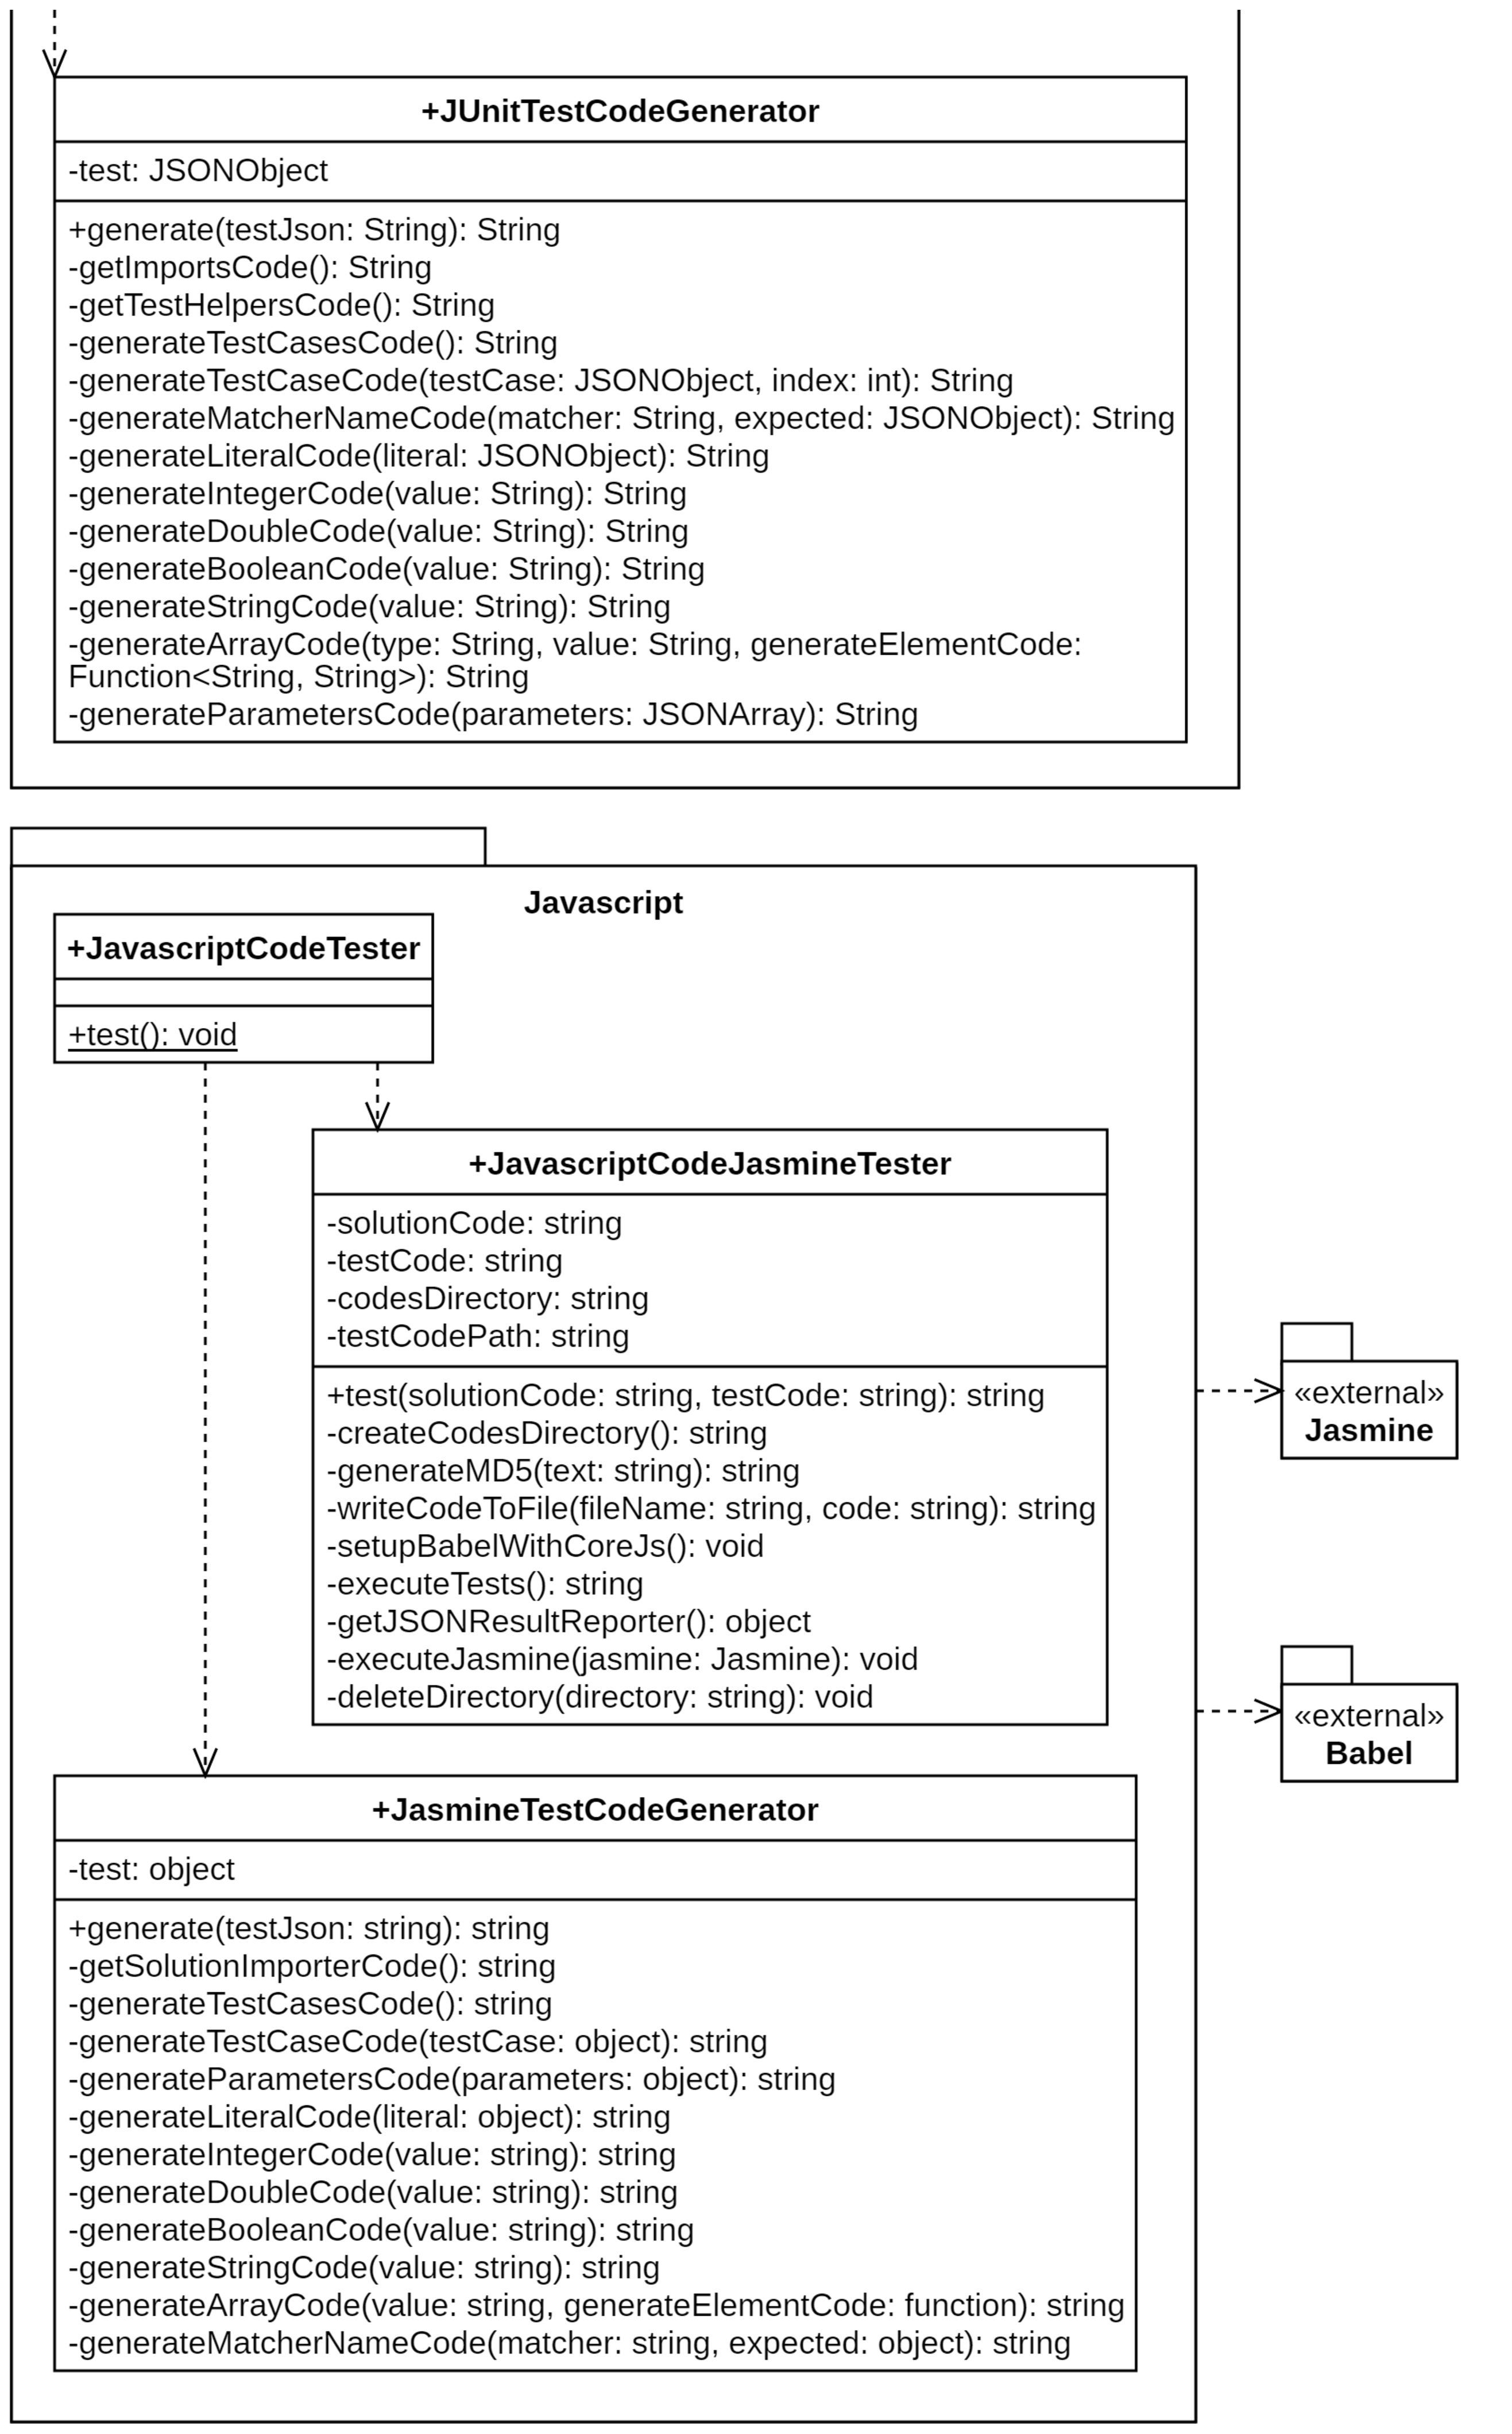
\includegraphics[scale=0.3333]{staruml/tester-system-class-diagram-2}
				\caption{A tesztelő rendszer osztálydiagramja - 2. rész}
			\end{figure}
			
			\subsection{Egységteszt keretrendszer kódján alapuló tesztelés}
				Ez a tesztelési módszer egy, a feladat megoldására használt programozási nyelvvel együttműködő egységteszt keretrendszert használó tesztkód alapján történő tesztelésre használható. Szükséges hozzá a megoldás kódja, illetve az egységteszt keretrendszert felhasználó tesztkód.
				
				Ezt a módszert akkor használjuk, amikor a felhasználó maga írja a tesztkódot is, azaz a tesztvezérelt fejlesztés, illetve a ping-pong módszer (tesztvezérelt fejlesztés és páros programozás együttesen), mint szoftverfejlesztési módszerek használatával történő megoldáskor.
				
				Célja, hogy a tesztkódban lévő, a megoldást tesztelő teszteseteket lefuttatva jelentést kapjunk azok teljesüléséről.

				\subsubsection{A tesztelés közös lépései}
					\begin{enumerate}
						\item Megkapjuk a tesztelendő megoldás kódját, illetve a tesztkódot.
						\item Létrehozunk egy ideiglenes mappát, amiben a teszteléshez szükséges forráskódokat fogjuk tárolni. A mappa nevének egyedinek kell lennie. Ez biztosítja azt, hogy egyidejűleg több felhasználó is tudja használni az alkalmazást feladatok megoldására, ütközések nélkül. Ennek érdekében a mappanevet a következő minta adja: \texttt{\{HASH\}\_\{TIME\}}, ahol \texttt{\{HASH\}} a megoldás és a teszt forráskódok konkatenációjának az MD5 kódolási algoritmus által képzett kódja, illetve \texttt{\{TIME\}} a jelenlegi Unix-idő milliszekundumokban. Így azonos milliszekundumban is futtatható több tesztelés, amennyiben nem egyeznek meg teljesen a tesztelendő forráskódok.
						\item Kiírjuk a forráskódokat külön fájlokba az előbb létrehozott mappán belül. Egyes programozási nyelveknél fontos lehet, hogy hogyan nevezzük el a fájlokat, ezért erre figyelünk (lásd lentebb, az egyes nyelvek sajátosságainál).
						\item Futtatjuk a tesztkódban lévő teszteket a megfelelő egységteszt keretrendszer segítségével. A teszteseteken belül történő futtatási hibák (exception) esetén sikertelennek nyilvánítjuk az érintett teszteseteket, nem állunk meg a teszteléssel. Bármilyen más, a tesztelés folytatását lehetetlenné tevő hiba (pl. szintaktikai vagy fordítási hiba) esetén megszakítjuk a tesztelési folyamatot, hibával térünk vissza. A tesztek eredményeit egységes, általános formátumban szeretnénk megkapni, erre a JSON szabványt használjuk. Ennek érdekében felüldefiniáljuk az egységteszt keretrendszer alapértelmezett teszteredmény-jelentési módszerét. Ennek értelmében minden teszteset lefutása után legeneráljuk a keretrendszer által adott információk alapján az adott teszteset egységes eredményét, ami a teszteset nevéből és állapotából áll. Egy teszteset állapota lehet sikeres, sikertelen vagy kihagyott. Az összes tesztesetről előáll egy ilyen eredmény. Az így létrehozott JSON objektumot használjuk fel később az eredmények megjelenítésére a felhasználónak. A teszteredmények minta felépítése:
						\begin{minted}{json}
							[
								{ "name": "first test", "status": "pass" },
								{ "name": "second test", "status": "fail" },
								...
							]
						\end{minted}
						\item Végül töröljük a forráskódok tárolására használt ideiglenes mappát. Ezt akkor is megtesszük, ha bármelyik lépésben hiba történik.
					\end{enumerate}

				\subsubsection{Java tesztelés sajátosságai}
					\begin{itemize}
						\item A megoldás, illetve a tesztek fordításához és futtatásához az OpenJDK 14-es verzióját használjuk, egységteszt keretrendszernek pedig a JUnit 5-ös verzióját. A tesztelésre beküldött megoldás és teszt forráskódoknak meg kell felelniük az ezek által támasztott követelményeknek.
						\item Fontos szerepe van Java esetén, hogy a forrásfájlokat milyen néven mentjük el, ennek figyelmen kívül hagyása esetén a fordítási folyamat hibával térne vissza. Ha a forrásfájl osztálystruktúrájának legkülső szintjén van publikus osztály, interfész vagy felsorolási típus, akkor a fájl nevének meg kell egyeznie ennek a nevével. Egyéb esetben nincs megkötés a fájlnévvel kapcsolatban. Ezt a szabályt használjuk fel a fájlnév meghatározásakor. A forráskódban definiált osztálynevek kinyeréséhez a JavaParser Java forráskód elemzőt használjuk. A szintaktikai hibák detektálásához szintén a JavaParser-t használjuk.
						\item Le kell fordítanunk a Java forrásfájlokat, hogy használni tudjuk őket a tesztek futtatásakor. Ehhez a Java Compiler API-t használjuk, ami a Java fordítót használja fel. A lefordított fájlokat a forrásfájlokban opcionálisan deklarálható csomaginformáció szerinti konyvtárstruktúrába helyezzük, a forráskódok ideiglenes mappájába. Ebben a lépésben detektálni tudjuk a fordítási hibákat.
						\item A JUnitnak a tesztesetek lefuttatásához szüksége van az azokat tartalmazó osztályokra, mint objektumokra, és ehhez ezeknek az osztályoknak be kell töltve lenniük a tesztelő program használatára. Legtöbb Java program esetében már futtatáskor meg tudjuk adni az összes, a program által használandó osztályt. Itt nem ez a helyzet, mert a felhasználótól érkező megoldás és teszt csak a program futása alatt kerül használható formába, ezért ezeket futás alatt, dinamikusan kell betöltenünk. Ennek megoldására osztálybetöltőt használunk, amivel be tudjuk tölteni egy lefordított Java fájlokat tartalmazó mappából az osztályokat. Itt még nem vagyunk készen, ugyanis a betöltött osztályok közül meg kell keresnünk azokat, amelyek a felhasználó tesztkódjában lettek definiálva. Ehhez szükségünk van ezeknek az osztályoknak a teljes elérési neveire, ami nem más, mint a teszt forrásfájl osztálystruktúrájának legkülső szintjén lévő osztályok nevei, prefixálva az opcionális csomagnévvel. Ezeknek az információknak a kinyeréséhez szintén a JavaParser-t használjuk. Az így meghatározott elérési nevek alapján már meg tudjuk kapni a hozzájuk tartozó tesztosztályokat az osztálybetöltőből, amit így már fel tud használni a JUnit a tesztek futtatására.
					\end{itemize}

				\subsubsection{JavaScript tesztelés sajátosságai}
					\begin{itemize}
						\item A megoldás, illetve a tesztek futtatásához a Node.js 14-es verzióját használjuk, egységteszt keretrendszernek pedig a Jasmine 3-as verzióját. A tesztelésre beküldött megoldás és teszt forráskódoknak meg kell felelniük az ezek által támasztott követelményeknek.
						\item Bár JavaScript esetén a forráskódokat bármilyen néven elmenthetjük, a konvenció szerinti néven mentjük el őket, a megoldást \texttt{index.js}, a tesztet pedig \texttt{index.spec.js} néven. Ez segíti a megoldó felhasználót, hiszen így a tesztkódban, a megoldás importálásakor nem kell tudnia, hogy honnan kell importálnia, elegendő a jelenlegi mappa elérési útját megadnia, ami \texttt{"."}.
						\item Mivel Node.js 14-es verzióját használjuk a futtatáshoz, így azokat a JavaScript funkciókat, elemeket használhatja a felhasználó, amelyek ebbe be vannak építve. Ezt ki szeretnénk terjeszteni a legújabbakra, ennek érdekében Babel-t és Core.js-t használunk. A Babel feladata, hogy a felhasználó JavaScript forráskódját, amiben a legújabb JavaScript elemek is fel lehetnek használva, átalakítsa olyan JavaScript kóddá, ami működése alapján teljesen megegyezik, viszont az újabb nyelvi elemeket, amelyeket a JavaScriptet futtató környezet még nem támogat, helyettesíti más, megegyező működésű konstrukciókkal. A Core.js feladata pedig, hogy a felhasználó JavaScript kódjában lehetővé tegye olyan osztályok, függvények használatát, amelyek részei, vagy részei lesznek a JavaScript standard függvénytárának, de a futtató környezet még nem tartalmazza ezeket. Ezt úgy éri el, hogy a kódban helyettesíti a megfelelő osztály- és függvényhasználatokat azoknak a Core.js szerinti implementációjával. A felhasználónak a kódban nem kell tennie semmi különöset, a Babel és a Core.js olyan módon került beállításra, hogy a szükséges módosítások a felhasználó forráskódjában automatikusan megtörténnek azok betöltésekor.
						\item A Jasminenak a tesztek futtatásához a teszteseteket tartalmazó fájl elérési útjára van szüksége, amely rendelkezésünkre áll. Az esetleges szintaktikai hibák már a tesztek futtatásakor derülnek ki.
					\end{itemize}

			\subsection{Egységes formátumon alapuló tesztelés}
				Ez a tesztelési módszer programozási nyelv-független, egységes formátumú tesztesetek alapján történő tesztfuttatást tesz lehetővé. Ez azt jelenti, hogy ha van egy programozási feladatra egy-egy teljesen megegyező megoldásom két különböző programozási nyelven, illetve vannak ilyen, egységes formátumú teszteseteim ezekhez a megoldásokhoz, akkor bármely programozási nyelven írt megoldásra lefuttatva a teszteket, azonos eredményeket kapok. Ennek eléréséhez egy olyan, közös interfészre van szükség, amely minden támogatott programozási nyelven megvalósítható. Ennek értelmében a teszteket nem egy programozási nyelv kódjaként írjuk meg, hanem definiálunk egy sémát a JSON szabvány felhasználásával, amely sémában reprezentálni tudjuk a tesztjeinket. A tesztek futtatásakor ezt a JSON objektumot át kell alakítanunk a tesztelendő megoldás programozási nyelve szerinti egységteszt keretrendszer kódjává, amellyel már le tudjuk futtatni a teszteket. Ehhez a JSON struktúrában lévő adatoknak egyértelműen megfeleltethetőnek kell lenniük a cél egységteszt keretrendszerben használható konstrukciónak. Ehhez a módszerhez szükséges a megoldás kódja, illetve a egységes teszteket tartalmazó JSON struktúra.
				
				Ezt a módszert minden esetben használjuk, de más módon. Amikor a felhasználó csak a megoldás kódját írja, azaz normál mód, illetve páros programozás, mint szoftverfejlesztési módszer használatakor, akkor úgy használjuk ezt a módszert, hogy a feladatot létrehozó felhasználó által a létrehozáskor megadott egységes formátumú teszteket küldjük be tesztelésre a megoldó felhasználó megoldási kódjával együtt, amikor a felhasználó tesztelést kér. Egyéb esetekben, vagyis a tesztvezérelt fejlesztés és a ping-pong módszer, mint szoftverfejlesztési módszerek használatakor bár a felhasználó maga írja a tesztkódot is, de a megoldás tényleges megfelelőségének ellenőrzése céljából lefutnak a létrehozáskor meghatározott egységes formátumú tesztek is.
				
				A módszer célja, hogy a megoldáskor egységes formában meg tudjuk jeleníteni, hogy milyen elvárásoknak kell megfelelni, az egységes teszteseteket lefuttatva jelentést kapjunk azok teljesüléséről, illetve, hogy a feladatot létrehozó felhasználónak csak egyszer kelljen leírnia a teszteseteket és az működjön minden programozási nyelvvel.

				A JSON struktúra tartalmazza az egységes formátumú teszteseteket és a tesztelendő függvény meghívási kódját. Ez a kód nem más, mint ahogyan a megoldásfüggvényünket meghívnánk az adott programozási nyelven, de még paraméterek nélkül, és ezt a megoldó felhasználónak kell megadnia a tesztelendő függvény beazonosítása érdekében. A teszteseteknél minden egyes tesztesethez tartozik egy szöveges leírás, egy paraméterlista, egy összehasonlító művelet és az elvárt érték. Az összehasonlító művelet lehet egyenlőség- vagy nem-egyenlőség vizsgálat. A paraméterekhez és az elvárt értékhez tartozik egy típus és egy érték. Típus lehet egész szám, dupla pontosságú lebegőpontos szám, logikai érték, szöveges érték, egész számok tömbje, dupla pontosságú lebegőpontos számok tömbje, logikai értékek tömbje vagy szöveges értékek tömbje. Az értékeknek a típus által támasztott szabályoknak kell megfelelniük, a tömböknél az egyes elemek "|" karakterrel vannak elválasztva. Egy lehetséges minta felépítés:
				\begin{minted}{json}
					{
						"functionCallCode": "calculateSomething",
						"testCases": [
							{
								"description": "it should return the ...",
								"parameters": [
									{
										"type": "integer",
										"value": "2"
									},
									{
										"type": "string array",
										"value": "one|two|three|four"
									},
									...
								],
								"matcher": "not equals",
								"expected": {
									"type": "boolean",
									"value": "true"
								}
							},
							...
						]
					}
				\end{minted}

				\subsubsection{A tesztelés közös lépései}
					\begin{enumerate}
						\item Megkapjuk a megoldás kódját, illetve az egységes, JSON formátumú tesztadatokat.
						\item Az egységes formátumú teszteseteket átalakítjuk a megoldáshoz használt programozási nyelv szerinti egységteszt keretrendszert felhasználó tesztkóddá:
						\begin{enumerate}
							\item Beillesztünk olyan kódokat, amelyek beimportálják a tesztkód számára szükséges függőségeket, így lehetővé teszik használatukat. Ez programozási nyelvenként változik.
							\item Előállítjuk minden egységes tesztesetnek az egységteszt keretrendszerbeli megfelelőjét. Pontosan megfeleltetünk minden megadható összehasonlító műveletet, illetve literált az egységteszt keretrendszerben, illetve a programozási nyelvben használható megfelelőjével. A tömbliterálok megfeleltetésénél az egyes elemeinek meghatározásához azoknak a megfeleltetését használjuk fel. Szöveges literáloknál figyelünk arra, hogy a nyelv sajátosságainak megfelelően escapeljük a benne lévő karaktereket az előállított forráskódban, így bármilyen karakter használható értékként. Tömb literáloknál lehetőséget adunk arra, hogy az elválasztó karaktert is fel lehessen használni az értékekben azáltal, hogy az escapelt elválasztókat nem elválasztóknak, hanem annak megfelelő karaktereknek feleltetjük meg. Ezek használatával már meghatározhatóak a szöveges leírások, a paraméterlisták, az összehasonlító műveletek és az elvárt értékek, így felépíthetőek a tesztesetek kódjai.
						\end{enumerate}
						\item A így létrejövő teszt- és az eredeti megoldáskód felhasználásával ugyanaz a folyamat megy végbe, mint az egységteszt keretrendszer kódján alapuló tesztelés módszerénél.
					\end{enumerate}

				\subsubsection{Java tesztelés sajátosságai}
					\begin{itemize}
						\item Az átalakítás során a JUnitot felhasználó tesztkód kerül előállításra.
						\item Importálásnál szükségünk van a JUnitból felhasználandó elemekre és Java osztályokra.
						\item Az összehasonlító műveletek megfeleltethetőségének megkönnyítése érdekében legeneráljuk és beillesztjük a kódba olyan összehasonlító műveletek implementációját, amelyeket a JUnit nem tartalmaz, viszont szükségünk van rájuk az egységes formátum maradéktalan támogatása érdekében.
					\end{itemize}
								
				\subsubsection{JavaScript tesztelés sajátosságai}
					\begin{itemize}
						\item Az átalakítás során a Jasminet felhasználó tesztkód kerül előállításra.
						\item Be kell importálnunk a megoldás kódjában lévő, exportált elemeket. A JavaScript nem ad natív lehetőséget arra, hogy kizárólag a fájlnév alapján beimportáljunk abból mindent, fel kell tudnunk sorolni egyesével az importálandó elemeket. Ennek feloldásaként azt a trükköt alkalmazzuk, hogy olyan kódot illesztünk be a tesztkódba, amely lefutásakor lekérdezi a megoldás fájljából exportált elemek nevét és értékét, és ezeket felhasználva elérhetővé teszi őket a tesztkódban. A megoldás CommonJS és ES6 modulrendszert használva is működik.
					\end{itemize}

		\section{Fejlesztőkörnyezet}

			\subsection{Rendszerkövetelmények}
				A szerver, illetve a kliens futtatásához szükséges szoftverek:
				\begin{itemize}
					\setlength\itemsep{-0.5em}
					\item Docker futtatására alkalmas operációs rendszer (Windows, macOS vagy Linux)
					\item Docker Desktop (2.2.0.5 vagy újabb verzió)
					\item Make (opcionális) (3.81 vagy újabb verzió)
				\end{itemize}

				Az alkalmazás közvetlenül használt függőségei nem szükségesek, azok Docker konténerek segítségével állnak rendelkezésre.

			\subsection{Fejlesztőkörnyezet beállítása}
				Másoljuk a DVD melléklet tartalmát számítógépre, majd nyissunk egy terminál ablakot a szerver mappájában (\texttt{methcodus-server}). Indítsuk el a szerver telepítését:
				\mint{shell}|$ make all|

				Ezzel minden beállításra kerül, ami a szerver használatához szükséges:
				\begin{itemize}
					\item Létrejön a szerver futtatására képes Docker konténer, amely rendelkezik az alkalmazás által támogatott programozási nyelveken íródott forráskódok futtatásához szükséges szoftverekkel.
					\item A konténerben telepítésre kerülnek a tesztelő rendszerek függőségei, vagyis JavaScript esetén Jasmine és Babel, Java esetén pedig JUnit, JavaParser és JSON-Java, illetve lefordításra kerül a Java tesztelő kódja.
					\item A konténerben telepítésre kerülnek a szerver alkalmazás függőségei.
					\item Létrejön a MongoDB adatbázis futtatására képes Docker konténer.
					\item Elindul a két konténer. Egyik elindítja az alkalmazás szerverét a 3000-es porton fejlesztői üzemmódban, a másik pedig az adatbázis szervert. Ezután mindkét szerver elérhető lesz közvetlenül a konténereket futtató számítógépről is, illetve az alkalmazás szerver újra fog indulni fájlmódosítás esetén.
				\end{itemize}

				A szervert elérhetjük a \url{http://localhost:3000} címen, kipróbálhatjuk annak API-ját például egy API tesztelő szoftver segítségével. A terminálban lépjünk át a kliens könyvtárába (\texttt{methcodus-client}), és indítsuk el a kliens telepítését is:
				\mint{shell}|$ make all|

				Csakúgy mint a szerver esetében, ezzel minden előkészítésre kerül, ami a kliens használatához szükséges:
				\begin{itemize}
					\item Létrejön a kliens futtatására képes Docker konténer.
					\item A konténerben telepítésre kerülnek a kliens alkalmazás függőségei.
					\item Elindul a konténer. Elindítja az alkalmazás kliensét a 4200-as porton fejlesztői üzemmódban. Ezután elérhető lesz közvetlenül a konténert futtató számítógépről is, illetve az alkalmazás szerver újra fog indulni fájlmódosítás esetén.
				\end{itemize}

				Ezek után nyissuk meg egy böngészőben a \url{http://localhost:4200} oldalt, ahol elérhető és használható a kliens alkalmazás. A szerver, illetve a kliens alkalmazás mappájából kiadható néhány, fejlesztés közben hasznos parancs:
				\begin{center}
					\begin{tabularx}{\textwidth}{l>{\RaggedRight}X}
						\texttt{\$ make build} & az alkalmazást futtató konténer(ek) létrehozása/frissítése \\
						\texttt{\$ make install} & az alkalmazás konténerében a függőségek telepítése/frissítése \\
						\texttt{\$ make start} & az alkalmazás konténer(ei)nek elindítása \\
						\texttt{\$ make stop} & az alkalmazás konténer(ei)nek leállítása \\
						\texttt{\$ make destroy} & az alkalmazás konténer(ei)nek törlése \\
						\texttt{\$ make npm script=\{SCRIPT\}} & az alkalmazás konténerében a \{SCRIPT\} nevű npm script lefuttatása \\
						\texttt{\$ make ssh service=\{SERVICE\}} & az alkalmazás \{SERVICE\} nevű konténerjének shelljébe való belépés
					\end{tabularx}	
				\end{center}
				
		\section{Fejlesztési folyamat}

			\subsection{Konténerizálás}

				\subsubsection{Konténerek}
					Az alkalmazás szerverének és kliensének a fejlesztése konténerekben történik. Egy konténer \cite{containers} egy szabványos futtatható szoftveregység, ami tartalmazza egy alkalmazás kódját és annak a fejlesztéséhez és futtatásához szükséges összes függőséget, beleértve az operációs rendszert, a szükséges rendszereszközöket, beállításokat, illetve az alkalmazás fejlesztését és futtatását lehetővé tevő rendszereket. A fejlesztők becsomagolhatják az alkalmazásaikat konténerekbe, így a kód bármilyen környezetben futtatható. Általában érdemes arra törekedni, hogy egy konténer minél kisebb méretű legyen, amit úgy érhetünk el, hogy olyan operációs rendszert választunk kiindulásnak, ami nem tartalmaz túl sok olyan szoftvert, amit nem használ az alkalmazásunk, illetve csak olyan szoftvereket telepítünk, amelyeket az alkalmazásunk valamilyen formában felhasznál. Minden alkalmazásnak más lehet az ideális környezet és általában azt szeretnénk, hogy az alkalmazások függetlenül működjenek egymástól, ezért ajánlatos konténerenként csak egy alkalmazást futtatni. A konténerizált alkalmazások elszigeteltségük miatt általában gyorsabban és megbízhatóbban működnek, mint hagyományos társaik, illetve nem szükséges a használatukhoz semmilyen szoftver a konténereket futtatni képes platformon kívül. Ezen kívül pedig operációs rendszer függetlenek is az ilyen alkalmazások, minden infrastruktúrán ugyanúgy működnek.

					A konténerek operációs rendszeri folyamatizolációval és virtualizációval működnek, amelyek lehetővé teszik azt, hogy több alkalmazás komponens megossza egyetlen kernel erőforrásait. Ez nagyon hasonló elven működik, mint a virtuális gépeknél az erőforrások megosztása, viszont az operációs rendszer szintű absztrakciós rétegnek köszönhetően sokkal kisebb méretűek, az erőforrásokat hatékonyabban használják fel, illetve alkalmazásfejlesztésben egyszerűbben és gyorsabban felhasználhatóak.

					A Docker \cite{docker} egy nyílt forráskódú konténerizációs platform, segítségével konténereket hozhatunk létre és futtathatjuk azokat. Egy konténer leírása \texttt{Dockerfile} fájlban történik. Itt adhatók meg olyan konfigurációk, mint a kiindulási operációs rendszer, a konténer létrehozásakor a függőségek telepítéséhez és a rendszer megfelelő beállításához lefuttatandó shell parancsok, a forrás számítógépről a konténerbe átmásolandó fájlok és a konténer indításakor futtatandó shell parancs. Emellett megadható \texttt{docker-compose.yml} fájl is, amely többkonténeres alkalmazások definiálására, illetve a konténerek futtatásához kapcsolódó beállítások megadására szolgál, mint például környezeti változók megadása, a forrás számítógépről logikai meghajtók felcsatlakoztatása, portok és hálózatok definiálása. Dockert használunk a szerver és kliens alkalmazás konténerizálására. Mivel az alkalmazások teljeskörűen konténerizáltak, csak Dockerre van szükség a fejlesztéshez és futtatáshoz.

				\subsubsection{Az alkalmazás konténerizálása}
					Az alkalmazás három konténerből épül fel: adatbázis, szerver és kliens. A konténerek közös hálózatra vannak kötve, így el tudják érni egymást. Az alábbiakban ezen konténerek működése olvasható.

					Adatbázis:
					\begin{itemize}
						\setlength\itemsep{-0.5em}
						\item Az adatbázis konténere egy előre elkészített konténer, ami MongoDB 3.6.9 adatbázist futtat.
						\item Elérhetővé tesszük a konténerben futó adatbázishoz való hozzáférést a 27017-es porton.
						\item Az adatbázis adatainak tárolására megadunk egy kötetet.
					\end{itemize}

					Szerver:
					\begin{itemize}
						\setlength\itemsep{-0.5em}
						\item A szerver konténerizálásához az Ubuntu 18.04 operációs rendszerből indulunk ki.
						\item Telepítjük a Node.js 14-es verzióját, illetve az OpenJDK 14-es verzióját, amelyekre a tesztelő rendszereknek is, és magának az alkalmazásnak is szükségük van.
						\item Létrehozunk root jogokkal nem rendelkező felhasználót, ő fogja futtatni a szoftvert.
						\item Elérhetővé tesszük a konténerben futó alkalmazáshoz való hozzáférést a 3000-es porton.
						\item Beállítjuk a szükséges környezeti változókat, mint például a használandó portot, az adatbázis elérhetőségét és az engedélyezett klienseket.
						\item Felcsatoljuk a konténerbe az alkalmazás kódját tartalmazó mappát.
						\item Elindítjuk az alkalmazást fejlesztői módban.
					\end{itemize}

					Kliens:
					\begin{itemize}
						\setlength\itemsep{-0.5em}
						\item Szintén Ubuntu 18.04-ből indulunk ki.
						\item Telepítjük a Node.js 14-es verzióját, ami az alkalmazást futtatni fogja.
						\item Itt is létrehozzuk a root jogok nélküli felhasználót, elérhetővé tesszük a konténeren kívüli hozzáférést a 4200-as porton, beállítjuk a szerver elérhetőségét környezeti változóként, felcsatoljuk a kódot tartalmazó mappát, illetve elindítjuk az alkalmazás fejlesztői módját.
					\end{itemize}

			\subsection{Csomagkezelés}
				A csomagkezelés olyan tevékenység, amely során meghatározásra kerülnek, illetve beszerzésre kerülnek az alkalmazás futtatásához szükséges függőségek. Node.js alkalmazásokhoz a legelterjedtebb és legtöbb csomaggal rendelkező csomagkezelő rendszer az npm (Node Package Manager) \cite{npm}. Az npm esetén egy \texttt{package.json} nevű fájlban lehet meghatározni a függőségeket, scripteket lehet írni a fejlesztés könnyítése céljából, illetve különböző olyan beállításokat lehet megadni, amelyek leginkább akkor jönnek jól, ha közzé akarjuk tenni az alkalmazásunkat csomag formájában az npm-en. A függőségek megadhatók fejlesztési idejű függőségként vagy normál függőségként. Az npm egyben egy CLI eszköz is, amely a \texttt{package.json} fájlból dolgozva többek között telepíteni tudja az abban megadott függőségeket, illetve futtatni tudja a megadott scripteket. A szerver és a kliens alkalmazás függőségeinek kezelésére npm-et használ.
			
			\subsection{Verziókövetés}
				A Git \cite{git} egy nyílt forráskódú, elosztott verziókövető rendszer, egyben a legelterjedtebb mind nyílt forráskódú, mind kereskedelmi projektekre. A legtöbb operációs rendszerrel és fejlesztőkörnyezettel együttműködik, kiemelkedő teljesítménnyel rendelkezik.	Az alkalmazás fejlesztése során a Git verziókövető rendszert használtam. Három különböző repositoryt hoztam létre, egyik a szerver kódját tartalmazza (\texttt{methcodus-server}), másik a kliens kódját (\texttt{methcodus-client}), harmadik pedig a dokumentáció kódját (\texttt{methcodus-thesis}). A Conventional Commits specifikációt használtam a commit üzenetek strukturált megírására. A GitHub egy Gitet használó online verziókövető platform. GitHubot használtam a verziókövetés céljából, a repositoryk elérhetőek a \url{https://github.com/users/fityocsaba96/projects/1} címen.
			
			\subsection{Continuous Integration}
				A Continuous Integration (CI) \cite{ci} az a folyamat, amely a központi kódtárba került kódváltozásokat folyamatosan, automatizáltan képes letesztelni és amennyiben az megfelel a támasztott követelményeknek, továbbítja a Continuous Delivery (CD) folyamatnak az éles rendszerbe való integrálás céljából. Egy ilyen rendszer úgy működik, hogy amikor kódváltozást észlel (például új commit érkezik a verziókövető rendszerbe), akkor előkészít egy megfelelő környezetet a kód futtatására a kód legfrissebb változatával együtt, és lefuttat a kóddal kapcsolatban előre megadott parancsokat, amelyekkel a kód működését, minőségét ellenőrzi. Ezek sikertelensége esetén nem történik semmi, ellenkező esetben viszont a kód egy CD folyamatnak lehet átadva, ahol kikerül éles környezetbe, használatra kész állapotra lesz hozva. Ezt nevezzük deploymentnek.

				A Codeship \cite{codeship} egy hosztolt, felhőalapú, CI folyamatokat támogató szolgáltatás. Codeshipet használunk mind a szerver, mind a kliens alkalmazás esetén. Amikor commit érkezik a GitHub repository master ágába, lefuttatja a CI folyamatot. A következőkben az alkalmazás CI folyamatai olvashatók.

				Szerver:
				\begin{itemize}
					\setlength\itemsep{-0.5em}
					\item Lemásoljuk a legfrissebb kódbázist egy elkülönített környezetbe.
					\item Telepítjük a Node.js 14-es verzióját, illetve az OpenJDK 14-es verzióját, amelyekre a folyamat további lépéseiben szükségünk van.
					\item Telepítjük az alkalmazás függőségeit. Ezek cachelésre kerülnek, azaz legközelebb nem kell minden függőséget újra telepíteni.
					\item Lebuildeljük az alkalmazást, hogy például a fordítást hibákat és egyéb figyelmetlenségeket kiszűrjük.
					\item Statikus kódellenőrzést futtatunk TSLint segítségével, amellyel stilisztikai, esztétikai és kódminőségi hibákat szűrhetünk ki.
					\item Lefuttatjuk az alkalmazáshoz írt egységteszteket, amivel biztosítjuk a tesztelt egységek megfelelő működését.
					\item Átadjuk a működő kódbázisunkat a Herokunak, ahol az deployolásra kerül.
				\end{itemize}

				Kliens:
				\begin{itemize}
					\setlength\itemsep{-0.5em}
					\item Szintén lemásoljuk az új kódbázist.
					\item Telepítjük a Node.js 14-es verzióját, amelyekre a folyamat további lépéseiben szükségünk van.
					\item Itt is telepítjük a függőségeket, lebuildeljük az alkalmazást, lefuttatjuk a statikus kódellenőrzést, illetve átadjuk a kódbázist deployolásra.
				\end{itemize}
			
			\subsection{Continuous Delivery}
        A Continuous Delivery (CD) \cite{cd} az a folyamat, amely a kódváltozásokat folyamatosan, automatizáltan képes integrálni az éles rendszerbe olyan módon, hogy az integráció után azonnal az új rendszer áll a felhasználók rendelkezésére a régi helyett. Egy CI rendszerrel kombinálva ennek az az eredménye, hogy amint új, helyesen működő kód kerül beküldésre, a felhasználók azt szinte azonnal, automatikusan megkapják, így mindig a működő legfrissebb változatot használhatják és nem kell hosszú időket várni az egyes újabb verziók megjelenésére. Egy ilyen rendszer úgy működik, hogy amikor valamilyen forrásból új forráskódot kap vagy kódváltozást észlel a hozzákapcsolt verziókövető rendszerben, akkor deployolja azt, vagyis előkészíti a megfelelő éles környezetet a kód futtatására a kód legfrissebb változatának felhasználásával, lebuildeli az alkalmazás éles környezetben használandó változatát, elindítja a lebuildelt alkalmazás kiszolgálását, utolsó lépésként pedig megjelenteti az alkalmazást, így ezután már az új változat fog betöltődni az alkalmazás webcímén.

        A Heroku \cite{heroku} egy felhőalapú, CI/CD folyamatokat támogató alkalmazás platform szolgáltatás (PaaS). Támogatja a legismertebb programozási nyelvek futtatását, ám lehetőségünk van saját, Docker alapú futtatókörnyezet használatára is. Herokun minden alkalmazás elkülönített, könnyűsúlyú konténerekben, úgynevezett dynokban fut. Bekapcsolható sok különböző kiegészítés, amelyekkel például adatbázis, monitorozási vagy üzenetküldési szolgáltatásokat adhatunk hozzá alkalmazásainkhoz. Herokut használunk a szerver, illetve a kliens alkalmazás CD folyamatainak megvalósítására, az éles alkalmazás kiszolgálására, illetve annak MongoDB adatbázis szolgáltatással való ellátására. Amikor megkapunk egy friss, működő kódbázist a Codeshiptől, lefut a CD folyamat. Az alkalmazás mindkét komponensének Herokun való futtatásához saját, Docker konténer alapú futtatókörnyezeteket használunk, amelyekben felépítjük az alkalmazások megfelelő futásához szükséges körülményeket. Erre azért van szükség, hogy az alkalmazás által támogatott programozási nyelveken íródott forráskódokat futtatni tudjuk. Ezen konténerek nagyon hasonló felépítésűek, mint a fejlesztésre használt változataik, ezzel minimalizáljuk az éles rendszerben fellépő váratlan hibákat. A kódbázisokban található egy-egy \texttt{heroku.yml} fájl, ezek írják le a Heroku számára, hogy hol találhatóak a futtatókörnyezetek definíciói, illetve hogy milyen kiegészítéseket szeretnénk használni, ez jelen esetben a szerver alkalmazás által használt adatbázis szolgáltatás. Az alábbiakban az említett futtatókörnyezetek működése olvasható.

        Szerver:
        \begin{itemize}
          \setlength\itemsep{-0.5em}
          \item A szerver konténerizálásához az Ubuntu 18.04 operációs rendszerből indulunk ki.
          \item Telepítjük a Node.js 14-es verzióját, illetve az OpenJDK 14-es verzióját, amelyekre a tesztelő rendszereknek is, és magának az alkalmazásnak is szükségük van.
          \item Létrehozunk root jogokkal nem rendelkező felhasználót, ő fogja futtatni a szoftvert.
          \item Átmásoljuk a konténerbe az alkalmazás kódját tartalmazó mappát.
          \item Telepítjük az alkalmazás függőségeit.
          \item Lebuildeljük az alkalmazást éles módban.
          \item Töröljük a kizárólag fejlesztéshez szükséges függőségeket.
          \item Elindítjuk az alkalmazást éles módban. A használandó portot, az adatbázis elérhetőségét és az engedélyezett klienseket előre beállított környezeti változókból kapjuk.
        \end{itemize}

        Kliens:
        \begin{itemize}
          \setlength\itemsep{-0.5em}
          \item Szintén Ubuntu 18.04-ből indulunk ki.
          \item Telepítjük a Node.js 14-es verzióját, ami az alkalmazást futtatni fogja.
          \item Itt is létrehozzuk a root jogok nélküli felhasználót, átmásoljuk a konténerbe a kód mappáját, telepítjük a függőségeket, lebuildeljük az éles alkalmazást, töröljük a nem szükséges függőségeket, illetve elindítjuk az alkalmazás éles módját, amelyhez a szerver elérhetőségét szintén környezeti változóként kapjuk.
        \end{itemize}

        Az éles kliens alkalmazás statikus fájlokból áll, kiszolgálásához egy saját, egyszerű szerver programot használunk. A szerver az Express nevű webalkalmazás keretrendszert használja fel kiszolgálásra, működése a következő:
        \begin{itemize}
          \setlength\itemsep{-0.5em}
          \item Hallgatunk a bejövő kérésekre környezeti változóban megadott porton keresztül.
          \item Amennyiben nem HTTPS-en keresztül érkezett a kérés, átirányítjuk azt HTTPS-re.
          \item Tömörítjük a válaszok törzsét egy külső modul segítségével.
          \item A statikus fájlokat az \texttt{index.html} kivételével (forrásfájlok, stíluslapok, képek) egyszerűen kiszolgáljuk az eredeti útvonalukon.
          \item Minden más útvonalon az \texttt{index.html} fájlt, vagyis magát az alkalmazást szolgáljuk ki. Kiszolgálás előtt beillesztünk a HTML kódba Cheerio segítségével egy scriptet, ami globális változóként definiálja a szükséges környezeti változókat a szerverről.
        \end{itemize}

        Az éles, Herokun futó szerver alkalmazás elérhető a \url{https://methcodus-server.herokuapp.com} címen, a kliens alkalmazás pedig a \url{https://methcodus-client.herokuapp.com} címen található.

			\subsection{Konfigurálás}
				A szerver, illetve a kliens alkalmazás tulajdonságainak konfigurálása a futtató rendszer környezeti változóinak felhasználásával történik. Ilyen tulajdonság például a szervernél az adatbázis elérhetősége, vagy a kliensnél a szerver elérhetősége. Környezeti változókat használni előnyösebb, mint konfigurációs fájlokat:
				\begin{itemize}
					\setlength\itemsep{-0.5em}
					\item Nem kerül be a konfiguráció a verziókövető rendszerbe, ezért szerveroldalon futtatott kód esetén a szenzitív konfigurációs adatok biztonságban maradnak.
					\item Teljesen elkülönül egymástól a forráskód és a konfiguráció, így kódváltozás nélkül módosíthatók a konfigurációs adatok.
					\item Ha egy alkalmazást több környezeten is fel szeretnénk állítani, csak a környezeti változókban lévő konfigurációt szükséges megváltoztatnunk.
				\end{itemize}

				A szerver alkalmazásban a Node.js egyszerű hozzáférést biztosít a környezeti változókhoz. A kliens esetén szintén a szerveren lévő környezeti változókra lenne szükségünk, de ehhez nem tudunk hozzáférni valós időben. Ennek megoldásaként a kliensbe belecsomagoljuk az aktuális környezeti változókat. Csak az \texttt{environment.json} fájlban megadott nevű környezeti változókat gyűjtjük ki a kliens számára. Erre azért van szükség, mert nem szeretnénk nem releváns, esetleg szenzitív adatokat hozzáférhetővé tenni a kliensen. Fejlesztői mód használatakor egy Webpack plugin segítségével globális változóként definiáljuk a kigyűjtött környezeti változókat a buildelés részeként. Ehhez képest éles módban a már említett, HTML kódba szúrt globális változón keresztül érjük el a környezeti változókat.
		
		\section{Tesztelés}
			Az alkalmazás tesztelése két részben történt; készültek egységtesztek, illetve manuális tesztek.

			\subsection{Egységtesztek}
				Az egységtesztek \cite{unittesting} az alkalmazást felépítő apró szoftverkomponensek működését tesztelő tesztek. Ilyen teszteket általában úgy célszerű írni, hogy azzal a lehető legkisebb egységet teszteljük le, más komponens működését nem teszteljük. Ezekkel a tesztekkel biztosíthatjuk a már kész kódok helyes működését. Az egységtesztek fehér doboz tesztelésnek számítanak, hiszen a megírásukhoz ismerni kell a szoftver belső működését. A teszteseteket a komponensek bemeneti és kimeneti értékeinek dokumentációjának is tekinthetjük. 

				A megoldás tesztelő rendszerhez egységtesztek készültek. Ezek a tesztek minden részletét letesztelik mind az egységteszt keretrendszer kódján alapuló, mind az egységes formátumon alapuló tesztelési módszernek. A programozási nyelvektől független működésű tesztesetek Java és JavaScript nyelvek használata esetén is meg lettek fogalmazva, ezen kívül le lettek tesztelve a programozási nyelv-specifikus esetek is. A tesztek a \texttt{methcodus-server/src/tester/tester.service.spec.ts} fájlban találhatóak, összesen 60 darab egységtesztet tartalmaz. A tesztek írására a Jasmine nevű egységteszt keretrendszert használtam. A leglényegesebb, letesztelt esetek a következőek:
				\begin{itemize}
					\item Egységteszt keretrendszer kódján alapuló tesztelés:
					\begin{itemize}
						\setlength\itemsep{-0.5em}
						\item Sikeres, sikertelen, illetve kihagyott állapotú tesztesetek
						\item Üres kód beküldése sikerrel, nulla teszteredménnyel végződik
						\item Egymásba ágyazott tesztstruktúrákon belüli tesztek is lefutnak
						\item JavaScript kódokban használható a CommonJS és az ES6 modulrendszer is, illetve minden modern JavaScript nyelvi elem és funkció
						\item Java kódokban használhatóak a csomagnevek
						\item Az ideiglenes forráskódokat tartalmazó mappa minden esetben kitörlődik
						\item Kivétel esetén sikertelen állapot
						\item Szintaktikai hiba, fordítási hiba és más hibák esetén hibaüzenet
					\end{itemize}
					\item Egységes formátumon alapuló tesztelés:
					\begin{itemize}
						\setlength\itemsep{-0.5em}
						\item Bármilyen támogatott paraméter típust elváró és önmagát visszaadó egyparaméteres függvény tesztelése a megfelelő eredménnyel zárul, bármely összehasonlító művelet esetén, igaz és hamis eredményt elváró esetekben is
						\item Nulla-, egy- és többparaméteres függvények is tesztelhetőek
						\item JavaScript megoldás kódból beimportáljuk, amik exportálva lettek
						\item Szöveges literálokat escapeljük, tömb literálokat escapelt elválasztó karakter esetén nem vágjuk el
					\end{itemize}
				\end{itemize}
			
			\subsection{Manuális tesztek}
			TODO (minden funkció lényegesebb kimeneteleire given-when-then leírás)
		
		\section{Továbbfejlesztési lehetőségek}
			Az alkalmazásban rengeteg lehetőség van még továbbfejlesztési szempontból. Ezek közül a legfontosabbak:
			\begin{itemize}
				\setlength\itemsep{-0.5em}
				\item Több programozási nyelv támogatása. A fejlesztés során ügyeltem arra, hogy a támogatott programozási nyelveket olyan módon kezeljem, hogy a jövőben egyszerűen beépíthetők legyenek további nyelvek.
				\item Csoportos feladatmegoldás élő menetben. Az egyéni gyakorláson kívül lehetőség lenne élő menethez csatlakozni, illetve indítani ilyet. Indítani egy már meglévő feladat és a használandó módszerek kiválasztásával lehetne. A csatlakozott felhasználók ezek használatával, illetve általuk választott programozási nyelvvel tudnának csatlakozni a feladatmegoldáshoz.
				\item Clean Code elvek, mint szoftverfejlesztési módszer támogatása. A többi módszerhez hasonlóan feladatok megoldásánál kiválasztható lenne módszerként ez is, és figyelmeztetne az alkalmazás, amikor nem tartja be a felhasználó a Clean Code elveit.
				\item Páros programozásnál élő chat a pár tagjai között.
				\item Részletesebb hibaüzenetek megjelenítése sikertelen tesztfuttatás, illetve sikertelen teszteredmény esetén.
				\item Egységes formátumon alapuló tesztelésnél több összehasonlító művelet (pl. kisebb, nagyobb, tartalmazás), illetve függvény paramétereknél és az elvárt értéknél több típus (pl. kulcs-érték párok, null) támogatása.
				\item Pont- és szintrendszer, ranglista. A feladatok megoldásáért járna pont, és egyre feljebb lehetne kerülni a ranglistán.
				\item Feladatmegoldásnál a kód írása közben automatikus mentés, később folytatható lenne a megkezdett feladat.
				\item A feladatoknál nehézség megadása, feladatok böngészésénél szűrési lehetőség nehézségre.
				\item Feladatok hozzáadása a kedvencekhez, a kedvenceknél ezen feladatok gyors elérése.
			\end{itemize}

	\begin{thebibliography}{99}

		\addcontentsline{toc}{chapter}{Irodalomjegyzék}

		\bibitem{tdd}
			Martin Fowler: Test Driven Development (2020.05.21.)
			\\\url{https://martinfowler.com/bliki/TestDrivenDevelopment.html}
		\bibitem{pairprogramming}
			Birgitta Böckeler, Nina Siessegger: On Pair Programming (2020.05.21.)
			\\\url{https://martinfowler.com/articles/on-pair-programming.html}
		\bibitem{containers}
			Stephen Guyton: Containers \& Containerization – Pros and Cons (2019.12.10.)
			\\\url{https://spin.atomicobject.com/2019/05/24/containerization-pros-cons}
		\bibitem{docker}
			IBM: What is Docker? (2019.12.10.)
			\\\url{https://www.ibm.com/cloud/learn/docker}
		\bibitem{npm}
			Nodejs.dev: An introduction to the npm package manager (2019.12.10.)
			\\\url{https://nodejs.dev/an-introduction-to-the-npm-package-manager}
		\bibitem{git}
			Atlassian: What is Git (2019.12.10.)
			\\\url{https://www.atlassian.com/git/tutorials/what-is-git}
		\bibitem{ci}
			Max Rehkopf: What is Continuous Integration (2019.12.10.)
			\\\url{https://www.atlassian.com/continuous-delivery/continuous-integration}
		\bibitem{codeship}
			Codeship (2019.12.10.)
			\\\url{https://codeship.com}
		\bibitem{cd}
			Martin Fowler: Continuous Delivery (2020.04.09.)
			\\\url{https://martinfowler.com/bliki/ContinuousDelivery.html}
		\bibitem{heroku}
			Heroku (2020.04.09.)
			\\\url{https://www.heroku.com/platform}
		\bibitem{unittesting}
			Software Testing Fundamentals: Unit Testing (2020.04.17.)
			\\\url{http://softwaretestingfundamentals.com/unit-testing}
		\bibitem{nodejs}
			Nodejs.dev: Introduction to Node.js (2020.04.18.)
			\\\url{https://nodejs.dev}
		\bibitem{typescript}
			TypeScript: What is TypeScript? (2020.04.18.)
			\\\url{https://www.typescriptlang.org}
		\bibitem{nestjs}
			NestJS: Introduction (2020.04.18.)
			\\\url{https://docs.nestjs.com}
		\bibitem{rest}
			Craig Buckler: An Introduction to REST and RESTful APIs (2020.04.18.)
			\\\url{https://www.sitepoint.com/developers-rest-api}
		\bibitem{mongodb}
			MongoDB: What Is MongoDB? (2020.04.18.)
			\\\url{https://www.mongodb.com/what-is-mongodb}
		\bibitem{angular}
			Aman Goel: Why should you learn Angular? (2020.04.18.)
			\\\url{https://hackr.io/blog/why-should-you-learn-angular}
		\bibitem{spa}
			MDN: SPA (Single-page application) (2020.04.18.)
			\\\url{https://developer.mozilla.org/en-US/docs/Glossary/SPA}
		\bibitem{codemirror}
			CodeMirror (2020.05.18.)
			\\\url{https://codemirror.net}
		\bibitem{express}
			freeCodeCamp.org: ExpressJS (2020.04.18.)
			\\\url{https://guide.freecodecamp.org/nodejs/express}
		\bibitem{test}
			TODO (kitölteni) (2020.04.06.)
			\\\url{http://example.com}

	\end{thebibliography}
	
	\chapter*{Mellékletek}

	\pagenumbering{gobble}
	\addcontentsline{toc}{chapter}{Mellékletek}

	\section*{DVD tartalma}
	TODO (tartalom, mappaszerkezet)

\end{document}
